% Expanded evidence supplement, revised 2 October 2026.
\documentclass[11pt]{article}
\usepackage[a4paper,margin=2.4cm]{geometry}
\usepackage[T1]{fontenc}
\usepackage{graphicx,amsmath,amssymb,booktabs,tabularx,longtable,array,xcolor}
\usepackage{tikz}
\usetikzlibrary{arrows.meta,positioning}
\usepackage[section]{placeins}
\usepackage{xr-hyper}
\usepackage[hidelinks]{hyperref}
\externaldocument[M-]{current_revised}
\graphicspath{{figures/}}
\renewcommand{\thesection}{S\arabic{section}}
\renewcommand{\thetable}{S\arabic{table}}
\renewcommand{\thefigure}{S\arabic{figure}}
\newcommand{\main}[1]{Section~\ref{M-#1} of the main text}
\definecolor{queryorange}{RGB}{145,80,0}
\newcommand{\authorquery}[1]{\par\smallskip\noindent\begin{minipage}{\linewidth}\color{queryorange}\textbf{[AUTHOR QUERY: #1]}\end{minipage}\par\smallskip}
\emergencystretch=2em
\setlength{\parskip}{3pt}
\title{Supplementary material\\[4pt]\large VCF-RDFizer: source-checkable semantic conversion for linked, policy-aware genomic querying}
\author{Elias Crum, Bart Buelens, Ruben Taelman, G\"okhan Ertaylan}
\date{}
\setcounter{topnumber}{4}
\setcounter{bottomnumber}{3}
\setcounter{totalnumber}{6}
\renewcommand{\topfraction}{.9}
\renewcommand{\bottomfraction}{.85}
\renewcommand{\textfraction}{.05}
\renewcommand{\floatpagefraction}{.7}
\begin{document}
\maketitle
\noindent This supplement preserves the experiment-level evidence behind the three questions in the main text. Sections~\ref{sup:repro}--\ref{sup:inputs} identify the evaluated builds and inputs; Sections~\ref{sup:model}--\ref{sup:validation} specify the representation and checks; Section~\ref{sup:usecase} gives the linked-query protocol; and Sections~\ref{sup:measurements}--\ref{sup:issues} retain measurements, configuration coverage and defects. Successful tests, negative tests, incomplete checks and unresolved oracle failures are distinguished.
\tableofcontents
\clearpage
\section{Reproducibility and execution}\label{sup:repro}

\textbf{Release and image.}
The tagged benchmark configuration uses VCF-RDFizer v3.1.0 (commit \texttt{d3b34d5}) from \texttt{ecrum19/vcf-rdfizer:v3.1.0}, with resolved image digest
\begin{center}\small\texttt{sha256:1904e96dde12ab2e2e70d8ee1267765c293ab100a8bd1b14d5b009b2bf8e34aa}\end{center}
\noindent
Image rebuilding is disabled during execution so that all cells in the tagged run use the same container.
The per-cell manifests retain the actual commit and image identifiers used for each measurement.
v3.1.0 bundles the VCF Core SHACL shapes from vocabulary commit \texttt{5bfd19d}.
The regional-retrieval cells postdate v3.1.0 (they need the regional runner and \texttt{tabix}) and were produced by commit \texttt{3da1a5a}.
The use case (\main{subsec:usecase}) converts with the v3.2.0 image and links and governs with pre-release builds of the linkers and policy plug-in, recorded per cell: uncommitted \texttt{feature/spdi-linker} trees on v3.2.0 (\texttt{f266db5}) for arms~1 and~2, each identified per cell by a recorded diff or tree hash, and commit \texttt{578c2be} for arm~3. v3.3.0 (commit \texttt{7ab2300}, image \texttt{sha256:1838720d\ldots06432}) releases them, adding two refusals that none of these runs meets: an empty selector list, and an RDF input with no VCF triples.

\textbf{Pinned toolchain.}
VCF-RDFizer v3.1.0 fixes its dependencies inside the container image: RMLStreamer 2.5.0, hdtc 1.1.0, pycottas 1.1.0, DuckDB 1.5.5, cyvcf2 0.34.0, pyshacl 0.30.1, Comunica 5.3.0 for N-Triples, \nolinkurl{@comunica/query-sparql-hdt} 5.0.1, the COTTAS Comunica engine 0.1.0, bcftools from the base distribution, and QLever pinned by image digest.
\texttt{rdf2hdt} and \texttt{hdt2rdf} are compiled from the hdt-cpp repository at image build time, so their exact revision is fixed by the image digest rather than by a version number; the resolved image for each benchmark run is recorded with its command and metrics.

\textbf{Hosts.}
Experiments run on two physically separate, identically specified hosts (\texttt{vcf-bench-1} and \texttt{vcf-bench-2}):
Ubuntu 24.04.4 LTS, kernel 6.8.0-85-generic, Intel Xeon Silver 4309Y at 2.80\,GHz (8 cores), 33.6\,GB RAM with swap disabled, a 210\,GB SSD, Docker 29.7.2, and Python 3.12.3.
Each complete experiment is assigned to one host and executed without concurrent benchmark jobs, keeping comparisons within-host.
On a shared calibration workload the two hosts produced the same graph: identical triple sets, a byte-identical COTTAS artifact and HDT index, and N-Triples and HDT files that differ only in line order and in the HDT header's \texttt{dcterms:issued} timestamp.
Their speed differed: the conversion phase took 26\,s on \texttt{vcf-bench-1} and 37\,s on \texttt{vcf-bench-2}, and validation 156\,s and 208\,s.
Timings are therefore compared only within a host; the calibration characterizes, rather than eliminates, variation between hosts.
Retrieval at scale (Table~\ref{tab:scale}) ran outside the campaign, on a third host, \texttt{vcf-bench-3}: the same CPU, 8 cores and 31.3\,GiB of RAM with swap disabled, under Ubuntu 22.04.5 and kernel 5.15. It queried graphs built by the published v3.1.0 image, with the validation runner of commits \texttt{245fe1f} (N-Triples) and \texttt{5ed75c8} (HDT and COTTAS), which select the thirteen core questions.

\textbf{What each cell records.}
The harness creates a fresh output directory for each cell and records its command, host, tool commit, container image, exit status, and wall time.
Tool reports provide stage timings, peak resident set size, triple counts, artifact sizes, and validation outcomes; workspace monitoring records transient disk use separately from final artifact size.
Input sizes used in performance comparisons are uncompressed VCF bytes, while the corpus table reports compressed download sizes.
Replicated comparisons report variability or confidence intervals; single-run corpus measurements describe the tested input and configuration without estimating run-to-run variation.
The per-cell records, normalized query results and comparison reports are recorded in the testing repository; a persistent archive of the complete evaluated snapshots is not yet deposited.

\textbf{The campaign.}
The campaign comprises 143 recorded cells over 96.2\,h of measured wall time (Table~\ref{tab:campaign}).
Every executed conversion cell records its own argv, host, tool commit and image digest, the two mutation-score cells their tool commit, and the integrated record of all cells is archived with the testing repository.
A non-zero exit is classified by what the cell asserted: two cells were required to be refused and were (\emph{refused}), two recorded an exit status without asserting an outcome (\emph{recorded}), and three were skipped by a stated guard.
No asserted expectation failed. This does not mean that all cells completed successfully: the status categories and denominator are retained below.

\begin{table}[!htbp]
\caption{The benchmark campaign, grouped by the question each experiment answers. \emph{Recorded}: a non-zero exit that the cell observed without asserting an outcome; \emph{refused}: the cell required the configuration to be rejected, and it was; \emph{skipped}: a guard refusal with a stated reason. Hosts: \texttt{vcf-bench-1} (b1), \texttt{vcf-bench-2} (b2). Every conversion cell was produced by the published v3.1.0 image; the two mutation-score cells ran the same commit's test harness on the host. Section numbers prefixed S are in this document; the others are in the main text.}\label{tab:campaign}%
\centering
\footnotesize
\setlength{\tabcolsep}{4pt}
\renewcommand{\arraystretch}{1.1}
\begin{tabularx}{\textwidth}{@{}l r >{\raggedright\arraybackslash}p{0.2\textwidth} c r >{\raggedright\arraybackslash}X@{}}
\toprule
\textbf{Experiment} & \textbf{Cells} & \textbf{Outcome} & \textbf{Host} & \textbf{Hours} & \textbf{Question answered} \\
\midrule
\multicolumn{6}{@{}l}{\textit{Conversion, scaling and storage}} \\
Records scaling            & 10 & all OK               & b1 & 10.99 & How cost grows with records (\S{}\ref{M-subsec3.3}) \\
Sample representation      & 30 & 29 OK, 1 skipped & b2 & 19.69 & How the two profiles grow with samples (\S{}\ref{M-subsec3.3}) \\
Storage mode               & 8  & all OK               & b1 & 12.87 & Peak workspace of plain vs space-optimized (\S{}\ref{M-subsec3.3}) \\
Corpus breadth             & 10 & 9 OK, 1 skipped      & b2 & 26.90 & HDT and COTTAS on ten public inputs (\S{}\ref{M-subsec3.4}) \\
\addlinespace
\multicolumn{6}{@{}l}{\textit{Input and configuration coverage}} \\
Representation axes        & 20 & all OK               & b1 & 4.82  & VCF 4.1--4.5; cost of INFO and header representations (\S{}\ref{sup:inputs}, \S{}\ref{sup:config}) \\
Difficult inputs           & 16 & 13 OK, 2 recorded, 1 skipped & b1 & 0.10 & Eleven awkward VCFs and the demonstration linkers (\S{}\ref{sup:inputs}) \\
Covering set               & 10 & all OK               & b1 & 0.35  & Every option value and pair (\S{}\ref{sup:config}) \\
Modes                      & 7  & all OK               & b1 & 0.03  & Each operating mode on its own (\S{}\ref{sup:config}) \\
Feasibility                & 9  & all OK               & b1 & 9.03  & Memory ceiling $\times$ configuration (\S{}\ref{sup:config}) \\
\addlinespace
\multicolumn{6}{@{}l}{\textit{Validation and retrieval}} \\
Robustness                 & 9  & all OK               & b1 & 0.25  & Determinism, round trip, mutation score (\S{}\ref{M-subsec3.5}, \S{}\ref{sup:validation}) \\
Equivalence                & 8  & 6 OK, 2 refused      & b2 & 6.84  & Four engines, both profiles, three artifacts (\S{}\ref{sup:config}) \\
Query cost                 & 6  & all OK               & b1 & 4.27  & SPARQL vs cyvcf2 on identical work (\S{}\ref{M-subsec3.6}) \\
\midrule
\textbf{Total}             & \textbf{143} & \textbf{136 OK, 2 recorded, 2 refused, 3 skipped} & & \textbf{96.16} & \\
\bottomrule
\end{tabularx}
\end{table}

\textbf{Distribution and maintenance.}
Each tagged VCF-RDFizer version is published across PyPI, Conda-Forge, and Docker Hub, so users can choose pip-, conda-, or container-based installation with matched versions, under the MIT License \cite{jimenez_2017_f1000}.
The GitHub README is the primary user guide: quick-start commands, end-to-end examples, command-line option documentation, and troubleshooting notes.
The project follows a release-oriented workflow with versioned release notes, public issue triage, and a unit-test suite that runs on Linux, macOS and Windows.


\subsection{Experiment-to-release ledger and unresolved archive fields}
The experiment families in Table~\ref{tab:release-ledger} must not be pooled into a single success rate or attributed to a single release. In particular, the 657.4M-triple conversion/retrieval graph and the 662.4M-triple normalized use-case graph are different artifacts.
\begin{table}[!htbp]
\caption{Build and assessment boundaries. A commit or image identifies executable state only if all local changes and external resources are also retained.}\label{tab:release-ledger}
\centering\small\setlength{\tabcolsep}{4pt}\renewcommand{\arraystretch}{1.1}
\begin{tabularx}{\textwidth}{@{}>{\raggedright\arraybackslash}p{0.24\textwidth}>{\raggedright\arraybackslash}p{0.27\textwidth}>{\raggedright\arraybackslash}X@{}}
\toprule
\textbf{Family} & \textbf{Recorded state} & \textbf{Assessment boundary}\\
\midrule
143-cell base campaign & v3.1.0, \texttt{d3b34d5}; full image digest above & Conversion, artifacts, fixtures, 984 applicable paired comparisons and configuration tests.\\
Regional retrieval & \texttt{3da1a5a} & Later runner with tabix; 11,160 regional executions.\\
Large-graph retrieval & v3.1.0 graphs; runners \texttt{245fe1f}, \texttt{5ed75c8} & Separate host; thirteen summary queries without SHACL.\\
Linked use case & v3.2.0 conversion; uncommitted pre-release trees on \texttt{f266db5} in arms 1--2; \texttt{578c2be} in arm 3 & SPDI, gene links and policy views. v3.3.0 \texttt{7ab2300} is the subsequent release, not the exact state of every run.\\
Review follow-ups & Default-profile mutation rerun; 250,000-record NG131FQA1I check & v3.1.0 (\texttt{d3b34d5}, image \texttt{sha256:1904e96d\ldots34aa}) on vcf-bench-2; QLever, expanded profile; the NG131FQA1I rerun without shapes; v3.1.0's size gates.\\
\bottomrule
\end{tabularx}
\end{table}
\authorquery{Archive the uncommitted arms 1--2 source trees and record the complete v3.3.0 image digest.}
The public vocabulary citation \cite{vcfc210} describes a separately versioned release. The shapes bundled with the base experiment are specifically commit \texttt{5bfd19d}; the two should not be silently treated as identical.

\section{Input and version coverage}\label{sup:inputs}

\textbf{The public corpus.}
Table~\ref{tab:test-corpus} lists the ten public VCFs. Download commands and canonical filename definitions are maintained in the testing repository.

\begin{table}[!htbp]
\caption{
  Public VCF corpus. File names are canonical \texttt{.vcf.gz} stems; later tables abbreviate the GIAB identifiers. Assembly and sample counts were verified from each file's header. Sizes are approximate compressed download sizes; the tool processes the uncompressed stream.}\label{tab:test-corpus}%
\centering
\footnotesize
\setlength{\tabcolsep}{4pt}
\renewcommand{\arraystretch}{1.1}
\begin{tabularx}{\textwidth}{@{}l l c r r >{\raggedright\arraybackslash}X@{}}
\toprule
\textbf{File} & \textbf{Provider} & \textbf{Assembly} & \textbf{Samples} & \textbf{MB (gz)} & \textbf{Evaluation role} \\
\midrule
\texttt{NG1N86S6FC}     & Sequencing.com  & GRCh38 & 1 & 379 & Consumer WGS \\
\texttt{NG131FQA1I}     & Dante Labs      & GRCh38 & 1 & 224 & Consumer WGS \\
\texttt{NB72462M}       & Nebula Genomics & GRCh38 & 1 & 341 & Consumer WGS \\
\texttt{60820188475559} & PGP upload      & GRCh37 & 1 & 325 & SNP-only profile \\
\texttt{60820188474283} & Dante Labs      & GRCh37 & 1 & 222 & Consumer WGS \\
\texttt{0GOOR\_HG002}   & precisionFDA    & GRCh38 & 1 & 69  & GIAB Truth Challenge v2 \\
\texttt{1000G\_phase3\_chr20} & 1000 Genomes & GRCh37 & 2{,}504 & 327  & Phased cohort \\
\texttt{HGSVC2}               & HGSVC2       & GRCh38 & 32      & 31.5 & Multi-sample SVs \\
\texttt{HG004\_GRCh38}        & GIAB v4.2.1  & GRCh38 & 1       & 149  & Benchmark genome, chr1--22 \\
\texttt{HG005\_GRCh38}        & GIAB v4.2.1  & GRCh38 & 1       & 139  & Benchmark genome, chr1--22 \\
\bottomrule
\end{tabularx}
\end{table}

\textbf{Declared VCF versions.}
Five single-purpose fixtures covering VCFv4.1 through VCFv4.5, plus one file with no \texttt{\#\#fileformat} declaration, all converted with exit code 0.
The generated RML mapping for each version is byte-identical apart from the asserted file class (\texttt{vcfc:VCF41File} through \texttt{vcfc:VCF45File}), which locates version awareness in the typed file resource rather than in field-level rules.
Field handling is therefore data-driven: the VCFv4.5 fixture's local-allele \texttt{FORMAT} keys (\texttt{LAA}, \texttt{LAD}) and the VCFv4.4 fixture's phase-set key (\texttt{PS}) are carried through as ordinary FORMAT entries, raising the per-record triple yield from 210 (4.4) to 252.5 (4.5) on otherwise matched two-record fixtures.
This is preservation, not interpretation: nothing in the graph resolves a local allele index to a global allele, so VCFv4.4/4.5 support is lexical carry-through pending a dedicated local-allele semantics layer.
The undeclared-version file also converted, via the documented fallback.

\textbf{Real cohorts.}
Nine of ten corpus inputs converted end to end (the first 250{,}000 records of eight files with headers retained, and \texttt{HG005\_GRCh38} whole), with HDT and COTTAS built and decode-checked for each.
The tenth, the 2,504-sample 1000 Genomes chromosome-20 call set, was skipped by the benchmark harness rather than refused by the tool: the harness withholds any corpus file with more than 1{,}000 sample columns from the expanded arm, because the expanded representation emits one call resource per record and sample.
Its full sample dimension was exercised instead through 10{,}000-record slices carrying all 2{,}504 samples, which converted in both representations; Section~\ref{sup:measurements} quantifies why the expanded arm cannot be run on the whole file at this disk budget.
The tool also applies a workspace check: before converting, it estimates the expanded workspace from the record and sample counts and refuses the run when that estimate exceeds three quarters of the free space, naming the condensed representation as the alternative.

\textbf{Difficult inputs.}
Eleven adversarial fixtures were run (Table~\ref{tab:awkward}; fixture files are named \texttt{awkward\_*} in the testing repository).
Nine converted and passed validation, including CRLF line endings, symbolic alleles, breakend ALT syntax, ploidy 4 and 3 in the same file, half-calls and haploid calls, missing values in every optional field, header keys declared but never used, the three-way \texttt{PASS}/\texttt{.}/failed-filter distinction, and a header-only file with no data records.
Two cells exited non-zero.
One is a refusal to convert: the truncated gzip stream, rejected in 0.58\,s at the decompression stage with a clear diagnostic, which is the intended behavior.
The sites-only file produced 245 triples and an HDT artifact, but its paired validation was not completed (Section~\ref{sup:issues}).

\begin{table}[!htbp]
\caption{Difficult-input fixtures. Outcomes are reported separately from validation. Neither a successful conversion nor an intended refusal establishes fidelity; the sites-only check is incomplete. Triple counts are for the complete graph the run produced.}\label{tab:awkward}%
\centering
\scriptsize
\setlength{\tabcolsep}{4pt}
\renewcommand{\arraystretch}{1.0}
\begin{tabularx}{\textwidth}{@{}>{\raggedright\arraybackslash}p{0.165\textwidth} >{\raggedright\arraybackslash}p{0.125\textwidth} r >{\raggedright\arraybackslash}p{0.135\textwidth} >{\raggedright\arraybackslash}X@{}}
\toprule
\textbf{Fixture} & \textbf{Outcome} & \textbf{Triples} & \textbf{Validation} & \textbf{Note} \\
\midrule
CRLF line endings & converted & 262 & PASS & No stray \texttt{\textbackslash r} in the last field's literal \\
Symbolic alleles & converted & 453 & PASS & \texttt{<DEL>} not treated as a base string \\
Breakend ALT & converted & 417 & PASS & Breakend ALT syntax preserved \\
Mixed ploidy & converted & 350 & PASS & Ploidy 4 then 3 followed the data \\
Half and haploid calls & converted & 446 & PASS & Four genotype cases stayed distinct \\
Missing values & converted & 321 & PASS & Missing-field fixture; missingness follows the field-specific representation \\
FILTER variants & converted & 486 & PASS & \texttt{PASS}, \texttt{.} and a failed code are three states \\
Declared FORMAT unused & converted & 293 & PASS & Header declaration represented although never used \\
Zero data records & converted & 189 & PASS & Header-only input; no data records \\
\midrule
Sites only & converted; validation not completed & 245 & incomplete & Graph and HDT artifact produced \\
Truncated gzip & refused at decompression & --- & not reached & Refused in 0.58\,s with a decompression diagnostic; intended \\
\bottomrule
\end{tabularx}
\end{table}


The successful sites-only frequency graph used in the linked case (Section~\ref{sup:usecase}) does not repair the malformed validation fixture. It establishes that the frequency-join workflow ran, not that a conformant sites-only input completed the full paired validation suite.

\section{Representation, related tools and implementation}\label{sup:model}
VCF-RDFizer emits RDF in the VCF Core Vocabulary (\texttt{vcfc:}, \url{https://w3id.org/vcf-core/vocab\#}) \cite{vcfc210}, a separately maintained vocabulary that models the VCF specification itself, version by version, for VCFv4.1 through VCFv4.5.
Its terms align with established resources for genomic coordinates (FALDO \cite{faldo_2016}), variant typing (the Sequence Ontology \cite{seq_ont_2005}), genotype and sample constructs (HERO \cite{hero-genomics_2025}), and features of the GA4GH VRS schema v2.0.1 \cite{ga4gh2025VRS}, so VCF-specific structure can be connected to existing terms.
The model preserves three information layers: file and header assertions, variant-record assertions, and sample and genotype assertions (Figure~\ref{fig2}).
The vocabulary carries classes, properties, domains and ranges but no OWL restrictions; value and cardinality constraints are SHACL shapes, which the validation layer applies (Section~\ref{M-subsec2.4}).

Sample-level data can be emitted in two profiles.
In the \emph{expanded} profile every sample value is its own resource, which makes genotypes directly queryable.
In the \emph{condensed} profile values are stored as sample-ordered vectors, reducing the number of RDF resources while requiring decoding for access to individual sample values.
Both profiles keep the same file, header and record context.
Let $V$ be the number of variant records, $S$ the number of samples, and $F$ the number of FORMAT keys per record.
For a uniform FORMAT layout, the expanded profile adds $VS$ sample-call resources and $VSF$ FORMAT-value resources, whereas the condensed profile adds $V$ cohort matrices and $VF$ value vectors.
Excluding the structure common to both, and assuming bounded ploidy and FORMAT-value arity, the sample-layer triple counts scale as
\begin{equation}
\begin{aligned}
T_{\mathrm{expanded}}  &= \mathcal{O}(S + VSF),\\
T_{\mathrm{condensed}} &= \mathcal{O}(S + VF).
\end{aligned}
\label{eq:sample-profile-scaling}
\end{equation}
The condensed profile removes the per-sample factor from the repeated RDF structure, but still stores all $VSF$ values inside vector literals, so its size in bytes keeps growing with $S$ even though its triple count does not (Section~\ref{M-subsec3.3}).

Core entities are minted from deterministic IRI templates over the source file and record position, so identifiers are reproducible but file-scoped: observations of the same variant in two files receive different IRIs. Identity across files is added by linking (Section~\ref{M-subsec:plugins}); GA4GH VRS computed identifiers \cite{ga4gh2025VRS} could serve beside NCBI SPDI and are future work.

\begin{figure}[!htbp]
\centering
\includegraphics[width=\textwidth]{vcf-core-classes.pdf}
\caption{\textbf{VCF Core Vocabulary, simplified class diagram.}
The backbone of the model VCF-RDFizer v3.1.0 emits, drawn from the ontology bundle it ships; all class and property names carry the \textit{vcfc:} prefix, \url{https://w3id.org/vcf-core/vocab\#}.
A \texttt{VCFFile}, typed with its version-specific subclass, links to three layers. In the \textbf{header} layer, header lines carry the INFO, FORMAT, FILTER, ALT and META definitions that values cite through \texttt{declaredBy}.
In the \textbf{record} layer, each \texttt{VCFRecord} has ordered alleles and a \texttt{VariantCall} carrying the INFO values, whose structured items retain their record, field and allele context.
In the \textbf{sample} layer, the call links either to per-sample \texttt{SampleCall}s, genotypes and allele calls (\emph{expanded} profile) or to one \texttt{CohortCallMatrix} of sample-ordered vectors (\emph{condensed} profile).
Structural-variant, phasing, local-allele and value-typing classes are omitted; the full vocabulary, with worked examples, is documented at \url{https://ecrum19.github.io/vcf-core-vocabulary/}.
} \label{fig2}
\end{figure}


\subsection{Documentation-based comparison and capability scope}
The comparison records the inspected documentation rather than a shared-input benchmark. An absent mark means a capability was not found in that documentation, not that the software cannot provide it. Package channels and mapping extensibility describe practical interfaces; they are not direct measures of semantic fidelity or usability.

\textbf{Related work.}
Earlier converters include the \textit{rdf-vcf} reader and the web-based \textit{VCF2RDF}, an isomorphic mapping to RDF/JSON-LD \cite{ruby_rdf_vcf,vcfr_2017}; a 2013 BioHackathon \textit{vcf2rdf} using FALDO and tool-specific terms \cite{katayama2019biohackathon}; and JVarkit's \textit{VcfToRdf}, TOGOvar's Rust \textit{VCF2RDF} and SPARQLing Genomics' \textit{vcf2rdf} \cite{JVarkit_2015,togovar_2022,sparqling_genomics_2020,sparqling_genomics_software}.
General tools also reach RDF: BioInterchange emits GFVO from GFF3, GVF and VCF 4.1--4.2 \cite{baran2015gfvo}, and \textit{bio-vcf} serializes through templates \cite{bio_vcf}.
Pipelines such as VariantKG build on these converters \cite{variantkg_2025}; AgroLD names a VCF2RDF component whose code was not located in the documentation assessment \cite{larmande2025agrold}; and Semantic Beacons exposes Beacon API responses as RDF through RML without materializing a file \cite{semantic_beac_2025}.
Table~\ref{tab:intro-tool-comparison} compares what these systems document; measuring conversion cost and fidelity against them on a shared input remains to be done.

\begin{table}[!htbp]
\caption{VCF-to-RDF converters and related semantic genomic-variation workflows, compared on the capabilities this study targets. Assessments are based on each system's publicly available documentation. This is a feature comparison, not a measured one: no other converter was run on the same input here, so the table shows what each system documents, not that one converts better or faster.}\label{tab:intro-tool-comparison}%
\centering
\footnotesize
\newcommand{\cY}{$\checkmark$}%
\newcommand{\cP}{($\checkmark$)}%
\newcommand{\cN}{--}%
\setlength{\tabcolsep}{3pt}
\renewcommand{\arraystretch}{1.15}
\begin{tabularx}{\textwidth}{@{}>{\raggedright\arraybackslash}X*{7}{c}@{}}
\toprule
\textbf{Tool / workflow} &
\textbf{CLI} &
\textbf{\shortstack{RDF\\model}} &
\textbf{\shortstack{Reprod.\\workflow}} &
\textbf{\shortstack{Metadata\\+ genotype}} &
\textbf{\shortstack{Extensible\\mappings}} &
\textbf{\shortstack{RDF\\compr.}} &
\textbf{\shortstack{Public\\release}} \\
\midrule
\multicolumn{8}{@{}l}{\textit{Dedicated VCF-to-RDF converters}} \\
\textbf{VCF-RDFizer (this study)} & \cY & \cY & \cY & \cY & \cP$^{c}$ & \cY & \cY \\
TogoVar VCF2RDF \cite{togovar_2022} & \cY & \cP & \cY & \cP & \cP & \cN & \cY \\
JVarkit VcfToRdf \cite{JVarkit_2015} & \cY & \cP & \cY & \cP & \cN & \cN & \cY \\
SPARQLing Genomics \cite{sparqling_genomics_2020} & \cY & \cP & \cY & \cY & \cP & \cN & \cP \\
VCF2RDF (web) \cite{vcfr_2017} & \cP & \cY & \cP & \cP & \cN & \cN & \cP \\
BioHackathon vcf2rdf \cite{katayama2019biohackathon} & \cY & \cP & \cP & \cP & \cN & \cN & \cP \\
\addlinespace
\multicolumn{8}{@{}l}{\textit{General genomic-format tools}} \\
BioInterchange \cite{baran2015gfvo} & \cY & \cY & \cY & \cP & \cN & \cN & \cY \\
bio-vcf \cite{bio_vcf} & \cY & \cN & \cY & \cP & \cY & \cN & \cY \\
ruby-rdf/rdf-vcf \cite{ruby_rdf_vcf} & \cY & \cN & \cP & \cP & \cN & \cN & \cY \\
\addlinespace
\multicolumn{8}{@{}l}{\textit{Knowledge-graph construction pipelines}} \\
VariantKG$^{a}$ \cite{variantkg_2025} & \cP & \cP & \cP & \cY & \cN & \cN & \cP \\
AgroLD VCF2RDF$^{b}$ \cite{larmande2025agrold} & \cN & \cP & \cN & \cN & \cN & \cN & \cP \\
\addlinespace
\multicolumn{8}{@{}l}{\textit{Virtual semantic access}} \\
Semantic Beacons \cite{semantic_beac_2025} & \cN & \cP & \cP & \cP & \cY & \cN & \cP \\
\bottomrule
\end{tabularx}
\vspace{1mm}
\parbox{\textwidth}{\footnotesize\raggedright \cY{}~supported and documented; \cP{}~partial or limited; \cN{}~not found in public documentation.
\textbf{CLI}: command-line use in pipelines.
\textbf{RDF model}: documented vocabulary for the output.
\textbf{Reprod.\ workflow}: documented, reproducible VCF-to-RDF route.
\textbf{Metadata + genotype}: header metadata kept with genotype and sample data.
\textbf{Extensible mappings}: rules editable without changing the converter.
\textbf{RDF compr.}: integrated compressed RDF output.
\textbf{Public release}: distributed package, executable or container.\\[1pt]
$^{a}$Converts VCF through SPARQLing Genomics' vcf2rdf after SnpEff annotation, then adds its own ontology for CADD scores and patient metadata.
$^{b}$Named in \cite{larmande2025agrold} as part of the AgroLD ETL; the assessment reflects public documentation inspected in September 2026.
$^{c}$RML maps the record backbone, about 5\% of the triples; the content-bearing layers (samples, INFO, QUAL, header) come from the wrapper's emitters, configured by options rather than mappings (Section~\ref{M-subsec2.2}).}
\end{table}
\begin{table}[!htbp]
\caption{VCF-RDFizer capability status and benchmark scope. ``Supported'' describes the release; the evaluation column states what this study measured, so that support is not mistaken for evidence. Section numbers without the S prefix are in the main text.}\label{tab:capabilities-summary}%
\centering
\scriptsize
\setlength{\tabcolsep}{3pt}
\renewcommand{\arraystretch}{0.96}
\begin{tabularx}{\textwidth}{@{}>{\raggedright\arraybackslash}p{0.2\textwidth}>{\raggedright\arraybackslash}p{0.15\textwidth}>{\raggedright\arraybackslash}p{0.15\textwidth}>{\raggedright\arraybackslash}X@{}}
\toprule
\textbf{VCF component / capability} & \textbf{Release} & \textbf{Evaluation} & \textbf{Notes / limitations} \\
\midrule
Core record fields (CHROM, POS, ID, REF, ALT, FILTER) & Supported (v3.1.0) & Validated & Q1--Q4 equal in completed comparisons; the broader suite has the follow-up failures reported in the main text (Section~\ref{M-subsec3.5}) \\
QUAL & Supported & Q11 record digest & Typed literal for every record; a missing QUAL is \texttt{vcfc:Null} \\
INFO & Supported; structured by default & Q11 and Q12 digests & Typed value per record and key, per-allele items for Number=A/R/G, plus the complete \texttt{infoRaw} string \\
FORMAT and sample/genotype values & Supported & Q5--Q6 exact; Q13 digest & Half-calls, haploid calls and ploidy 4/3 survive conversion (Table~\ref{tab:awkward}); called allele, sample index and phasing require the deeper shapes for the tested mutations \\
HEADER metadata & Supported & Census queries and shapes & Header attribute-value agreement requires the deeper shapes, not merely the default profile \\
Multi-sample conversion & Supported & Measured, 1--2{,}504 samples & Condensed adds 5 triples per sample; expanded adds 25 per sample per record (627M triples for 10{,}000 records at 2{,}504 samples), so the whole cohort was converted in neither (Section~\ref{M-subsec3.3}) \\
Structural and symbolic alleles & Lexically supported & HGSVC2 converted; Q2 passes on symbolic and breakend fixtures & ALT remains the source lexical field; allele-value mutations are caught only by the full shape profiles \\
Queryable HDT, COTTAS & Supported & Measured & 118 HDT and 34 COTTAS artifacts, all decode checks passed; COTTAS smallest throughout (Section~\ref{M-subsec3.4}) \\
Gzip/Brotli packaging & Supported & Covering set (Section~\ref{sup:config}) & Packages must be unpacked before querying; no codec comparison \\
Policy annotations & Plug-in v0.2.0 with v3.3.0 & Real genomes, up to a whole genome & ODRL on files and declared graph selections, DUO purposes; every view checked against a VCF-side oracle; simulated consents, single-sample files; governed release, not anonymization (Section~\ref{M-subsec:usecase}) \\
External linking & SPDI, Ensembl-gene and MyVariant linkers with v3.3.0 & Real genomes & SPDI joins eligible alleles under the stated reference/normalization assumptions; tier~3 confirmed 92--93\% of rsID rewrites (Section~\ref{sup:usecase}) \\
\bottomrule
\end{tabularx}
\end{table}
\subsection{Conversion and incremental representation construction}\label{sup:construction}
Conversion has five stages:
(1) each VCF is split into record, header-line and file-metadata TSV logical sources;
(2) modular RML rule sets \cite{rml_2024}, authored in Turtle and executed by RMLStreamer \cite{rmlstreamer_2022}, map them to RDF;
(3) emitters add the remaining fields and the samples, and every part is appended to one N-Triples aggregate;
(4) optional gzip or Brotli packages and queryable HDT and COTTAS representations are built from the aggregate; and
(5) every representation is validated, packaged and reported.
Options keep these concerns separate (\texttt{--rdf-storage-mode}, \texttt{--rdf-compression}, \texttt{--representations}, \texttt{--artifact-compression}), so an \texttt{.hdt} or \texttt{.cottas} file can be kept for querying while a \texttt{.gz} or \texttt{.br} package is made for transport.

RML maps the record backbone: nine triples per record, 5.3\% of the HG005 graph's triples. The content-bearing layers --- samples, structured INFO, QUAL and the header, 94.7\% of that graph --- come from the tool's emitters, configured by options, because the implemented mapping path delegates per-value datatype selection to emitters (a missing QUAL, for instance, is written \texttt{"."\textasciicircum\textasciicircum vcfc:Null}). The TSV step exists because VCF is not a native RML logical source.

In \texttt{plain} storage mode the parts are appended to one uncompressed \texttt{.nt} graph; in \texttt{space-optimized} mode each part is gzip-compressed and appended as a member of one concatenated-gzip \texttt{.nt.gz} stream, which standard gzip readers expose as one N-Triples sequence. Either way each part is deleted once appended, so all parts and a full uncompressed aggregate never coexist.

HDT and COTTAS are built one record-safe chunk at a time, so at most one uncompressed chunk exists while they are built. HDT parts are produced with \texttt{rdf2hdt} \cite{hdtcpp,hdt_2013}, merged pairwise with \texttt{hdtc} \cite{hdtc_2026,Diefenbach2020HDTCat} and indexed. COTTAS parts are produced with pycottas \cite{pycottas_2026} and merged in one streaming $k$-way pass with an \texttt{spo} index (v3.2.0 adds the other orders); COTTAS files are queried by a Comunica engine that evaluates SPARQL over the Parquet table with DuckDB \cite{comunica_cottas_2026}. Before the raw RDF is removed, every artifact is decoded with its native reader and its triple count compared with the source's; a mismatch fails the run. The following subsection details chunking.


\begin{figure}[!htbp]
\centering
\includegraphics[width=\textwidth]{vcf2rdf-v3.pdf}
\caption{\textbf{VCF-RDFizer v3.1.0 pipeline.}
\textbf{(1) Conversion}: the VCF is split into three TSV logical sources; RMLStreamer applies the RML rules to emit VCF Core N-Triples, and direct emitters add the row-dependent fields whose datatype is chosen per value (QUAL, ID, FILTER, alleles, structured INFO) and the samples in the \emph{expanded} or \emph{condensed} profile.
Every part is appended to one aggregate and then deleted: a plain \texttt{.nt} file, or in space-optimized mode a concatenated-gzip \texttt{.nt.gz} stream.
\textbf{(2) Queryable representations}: the aggregate is read incrementally and only one record-safe raw chunk exists at a time; \texttt{rdf2hdt} and pycottas each consume it before it is deleted.
HDT parts are merged pairwise in a balanced tree with \texttt{hdtc} and indexed; COTTAS parts are merged in one streaming $k$-way pass with an \texttt{spo} index.
\textbf{(3) Validation and packaging}: each artifact is decoded back and its triple count compared with the source; the graph is then checked against the VCF Core SHACL shapes and against thirteen questions answered both by SPARQL and by a VCF parser.
HDT and COTTAS files are queryable as written; gzip or Brotli packages are for transport and must be unpacked before querying.
} \label{fig1}
\end{figure}
\textbf{Chunked construction of HDT and COTTAS.}
The representation stage reads the plain or gzip aggregate incrementally, respects newline-terminated N-Triples record boundaries, and materializes one raw chunk in a Docker-managed workspace.
Each selected representation builder consumes that chunk before it is deleted and the next one is created (Figure~\ref{fig:chunks}).
At most one uncompressed RDF chunk exists at a time; the final parts, merge intermediates, indexes and converter scratch space still require storage, but no full decompressed duplicate of the aggregate is created.
HDT chunks are converted with \texttt{rdf2hdt} from hdt-cpp \cite{hdtcpp,hdt_2013} and merged pairwise in a balanced tree with \texttt{hdtc create} \cite{hdtc_2026}, which performs the same logical merge as HDTCat \cite{Diefenbach2020HDTCat} under a fixed memory budget and without Java; an unpaired file is carried into the next round, and each merge's scratch directory is removed as soon as that merge completes.
The final HDT is indexed by \texttt{hdtc}, producing the sibling \texttt{.hdt.index.v1-1} index without executing a query; intermediate indexes are not retained.
COTTAS chunks are converted with pycottas \cite{pycottas_2026} and merged in one streaming $k$-way pass rather than pairwise, so no global in-memory hash table or full-size temporary spill is built.
In v3.1.0 the merged output carries a fixed \texttt{spo} index; v3.2.0 adds the other index orders.
Each COTTAS operation runs in an isolated temporary working directory, so that its local DuckDB scratch database cannot be reused by a later chunk or merge.
Chunk conversion, merging, final indexing, validation, and packaging are timed separately.

\begin{figure}[!htbp]
\centering
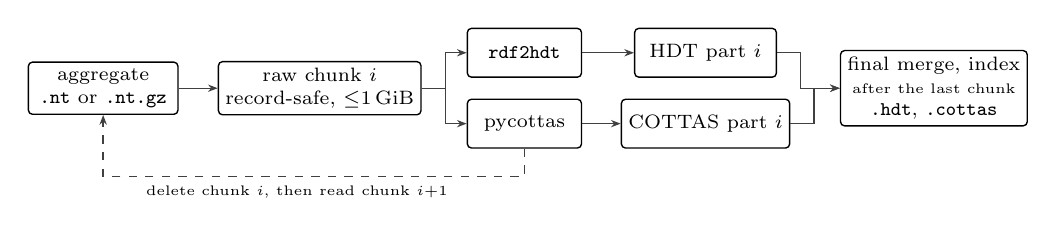
\begin{tikzpicture}[
  font=\scriptsize, >={Stealth[length=3.5pt]},
  st/.style={draw, rounded corners=1.5pt, align=center, inner sep=2.5pt, minimum height=0.62cm, line width=0.5pt, font=\scriptsize},
  fl/.style={->, line width=0.5pt, draw=black!75},
]
\node[st, minimum width=1.9cm] (agg) at (0,0) {aggregate\\\texttt{.nt} or \texttt{.nt.gz}};
\node[st, minimum width=2.1cm] (chk) at (2.75,0) {raw chunk $i$\\record-safe, $\leq$1\,GiB};
\node[st, minimum width=1.45cm] (h) at (5.35,0.45) {\texttt{rdf2hdt}};
\node[st, minimum width=1.45cm] (c) at (5.35,-0.45) {pycottas};
\node[st, minimum width=1.8cm] (hp) at (7.65,0.45) {HDT part $i$};
\node[st, minimum width=1.8cm] (cp) at (7.65,-0.45) {COTTAS part $i$};
\node[st, minimum width=1.9cm] (fin) at (10.55,0) {final merge, index\\{\tiny after the last chunk}\\\texttt{.hdt}, \texttt{.cottas}};
\draw[fl] (agg) -- (chk);
\draw[fl] (chk.east) -- ++(0.3,0) |- (h.west);
\draw[fl] (chk.east) -- ++(0.3,0) |- (c.west);
\draw[fl] (h) -- (hp); \draw[fl] (c) -- (cp);
\draw[fl] (hp.east) -- ++(0.3,0) |- (fin.west);
\draw[fl] (cp.east) -- ++(0.3,0) |- (fin.west);
\draw[fl, dashed] (c.south) -- ++(0,-0.35) -| node[pos=0.27, below, font=\tiny]{delete chunk $i$, then read chunk $i{+}1$} (agg.south);
\end{tikzpicture}
\caption{One chunk at a time: each record-safe chunk is consumed by every selected builder and deleted before the next is read.}\label{fig:chunks}
\end{figure}

\textbf{Chunk sizes.}
By default a chunk targets 512\,MiB of uncompressed N-Triples, bounded below by 128\,MiB and above by 1\,GiB (\texttt{--chunk-target-bytes}, \texttt{--chunk-min-bytes}, \texttt{--chunk-max-bytes}).
For constrained workspaces a lower-peak setting is 128\,MiB target, 64\,MiB minimum and 256\,MiB maximum, trading additional chunks and merges for a lower temporary peak.
Every experiment used the defaults except six cells of the memory-feasibility sweep, which used the lower-peak setting (Section~\ref{sup:config}).


\section{Validation specification, scope and sensitivity}\label{sup:validation}
\subsection{Queries and normalization}
Readable output need not be faithful output. The validation layer (\texttt{--validate}) therefore asks the graph thirteen standard VCF inspection and quality-control questions \cite{vcf_intro,BCFtools,cyvcf2_2017} in SPARQL, and derives each expected answer from the source VCF with cyvcf2, using \texttt{bcftools query} for exact FILTER text (Table~\ref{tab:semantic-queries}). Fourteen graph-integrity preflight queries run first: blank nodes, empty values, untyped missing tokens, the POS datatype, the cardinality of core record properties, the sample representation, the sample and genotype inventory, and the triple count.

\begin{table}[!htbp]
\caption{The thirteen-query equivalence workload. Each SPARQL result is normalized and must equal a result derived from the source VCF by the separate parser-based path (Q4's exact FILTER text via \texttt{bcftools query}). Ti/Tv, call rate and allele frequency are derived only after their underlying counts agree. Q11--Q13 count values in up to 256 buckets keyed on the first byte of SHA-256 over the IRI and values, which detects value changes that preserve ordinary counts but is not a collision-free proof of equality. For Q9, Q10, Q12 and Q13 the expected result follows the selected INFO and sample representations.}\label{tab:semantic-queries}%
\centering
\footnotesize
\setlength{\tabcolsep}{4pt}
\renewcommand{\arraystretch}{1.08}
\begin{tabularx}{\textwidth}{@{}>{\raggedright\arraybackslash}p{0.22\textwidth} >{\raggedright\arraybackslash}X@{}}
\toprule
\textbf{Query} & \textbf{Result compared, fields and scope} \\
\midrule
\multicolumn{2}{@{}l}{\textit{Record level --- every input}} \\
Q1\enspace Record density & Records per contig and 1-Mb window (\texttt{CHROM}, \texttt{POS}); checks coordinates and integer positions \\
Q2\enspace Allele shapes & Records per class --- SNV, multiallelic, insertion, deletion, substitution, symbolic/breakend, no ALT (\texttt{REF}, \texttt{ALT}) \\
Q3\enspace Ti/Tv & Transitions, transversions and biallelic SNVs; single-base A/C/G/T alleles only \\
Q4\enspace FILTER values & Records per exact FILTER string: \texttt{PASS}, \texttt{.}\ (not applied) or failed codes, combined codes kept whole \\
\addlinespace
\multicolumn{2}{@{}l}{\textit{Genotype level --- inputs with sample columns and \texttt{GT}}} \\
Q5\enspace Genotypes & Calls per sample and genotype class, including missing, haploid and other-ploidy calls; phased and unphased alike \\
Q6\enspace Allele counts & Sites per recomputed (AC, AN) pair; single-ALT sites with complete 0/1 haploid or diploid calls \\
\addlinespace
\multicolumn{2}{@{}l}{\textit{Metadata and graph structure}} \\
Q7\enspace File metadata & Exact \texttt{fileformat}, \texttt{reference} and \texttt{source} strings, with markers for absent declarations \\
Q8\enspace Header census & \texttt{\#\#} lines per header key (INFO, FORMAT, FILTER, contig, \dots) \\
Q9\enspace Predicate census & Triples per predicate against the counts expected from the VCF \\
Q10\enspace Class census & Resources per \texttt{rdf:type} against the expected inventory \\
\addlinespace
\multicolumn{2}{@{}l}{\textit{Value preservation --- IRI-bound digests}} \\
Q11\enspace Record digest & Records per bucket over each record's IRI, \texttt{CHROM}, \texttt{POS}, \texttt{ID}, \texttt{REF}, \texttt{ALT}, \texttt{QUAL}, \texttt{FILTER} and raw INFO \\
Q12\enspace INFO digest & Structured INFO values per bucket, bound to record and key; empty in raw-only INFO mode \\
Q13\enspace FORMAT digest & FORMAT values (expanded) or sample-ordered vectors (condensed) per bucket, beyond \texttt{GT} \\
\bottomrule
\end{tabularx}
\end{table}

Results must be exactly equal after normalization: strings for Q7 and integer counts elsewhere, including the digest buckets of Q11--Q13, which extend coverage to QUAL, INFO and FORMAT without guaranteeing value-by-value equality. The comparator keeps contig and sample identifiers, distinguishes \texttt{PASS} from \texttt{.}, and reports missing, extra and differing rows. Q5--Q6 apply only when the source has a \texttt{GT} field, and each input is validated only against its own graph, so inputs on different assemblies are never compared.

The same SPARQL text runs under four engines: QLever \cite{qlever_2017}, the default; Comunica over N-Triples (\nolinkurl{@comunica/query-sparql-file}) \cite{Taelman2018Comunica,comunica_file_docs_2026}; Comunica over HDT (\nolinkurl{@comunica/query-sparql-hdt}) \cite{comunica_hdt_docs_2026}; and the DuckDB-backed COTTAS engine \cite{comunica_cottas_2026}. Any engine can be pointed at any artifact, and \texttt{--validation-engine all} runs all four and records whether they agree. The layer also applies the vocabulary's SHACL shapes in three profiles. The default profile checks cardinality and datatypes; the other two check uniqueness and value agreement, and are costlier (Section~\ref{M-subsec3.5}).

What a passing comparison establishes is agreement of the specified summaries: a SPARQL engine and a VCF parser derive the same deterministic summaries from two representations of the same source. It does not establish that the source calls are biologically correct, normalized or concordant with a truth set.


\subsection{Scope of the campaigns}
The base campaign attempted validation 78 times and completed 76. It yielded 984 applicable query comparisons with no mismatches and four not-applicable genotype comparisons on the empty-input artifacts. Its paired checks ran on fixtures and slices up to 17.1M triples. The two malformed sites-only validations did not complete and are not successful comparisons.

The whole HG005 graph was decode/count checked in the corpus campaign. Separately, the retrieval experiment compared all thirteen QLever query answers at 657,425,805 triples with the parser, without SHACL (Table~\ref{tab:scale}). Those comparisons are not included in the 984 denominator. The 58.2M-triple consumer-genome follow-up is another separate run; it has three summary mismatches and must not be counted as a validation pass.

The default shape profile ran in 58 base validations, on graphs up to 0.96M triples, with no violations and 0.8--396.8\,s per run. Repeated conversion produced 17,098,746 triples with identical SHA-256 and no duplicate lines. A packaging round trip reproduced the digest and re-indexing left the artifact unchanged. These assess deterministic output under the tested conditions, not reproducibility of every later pre-release build.
\begin{table}[!htbp]
\caption{Validation evidence, grouped by the question each layer answers. Counts are pass/total, derived from archived reports. Sensitivity is measured on the defined fault set, not estimated for arbitrary faults.}\label{tab:validation-complete}%
\centering
\scriptsize
\setlength{\tabcolsep}{5pt}
\renewcommand{\arraystretch}{1.05}
\begin{tabularx}{\textwidth}{@{}>{\raggedright\arraybackslash}p{0.28\textwidth} r >{\raggedright\arraybackslash}X@{}}
\toprule
\textbf{Check} & \textbf{Passed} & \textbf{What it establishes} \\
\midrule
\multicolumn{3}{@{}l}{\itshape Is the graph faithful to the source VCF?}\\
N-Triples syntax (\texttt{rapper}) & 76/76 & The serialization parses \\
Paired SPARQL vs cyvcf2 (Q1--Q13) & 984/984\rlap{$^{\dagger}$} & Exact equality of normalized query results \\
Cross-check invariants & 1{,}144/1{,}144 & E.g.\ transitions $+$ transversions $=$ biallelic SNVs \\
Cross-engine agreement & 25/25 & Four-engine validations; 51 other completions used one engine \\
Native decode and triple count & 152/152 & 118 HDT, 34 COTTAS; source $=$ decoded \\
\addlinespace
\multicolumn{3}{@{}l}{\itshape Is the pipeline reproducible?}\\
Determinism, two runs & 1/1 & Identical SHA-256; 17{,}098{,}746 triples, 0 duplicate lines \\
Compress and decompress & 1/1 & Lossless through the packaging path \\
Index idempotence & 1/1 & Re-indexing does not perturb the artifact \\
\addlinespace
\multicolumn{3}{@{}l}{\itshape Would a fault actually be noticed?}\\
Injected faults caught, queries only & 96/113 \;(0.850) & 17 faults, spanning 10 mutation classes, are invisible to the queries \\
\quad with the default shape profile & 96/113 \;(0.850) & Cardinality and datatypes catch none of the 17 \\
\quad with all three shape profiles & \textbf{113/113} \;(1.000) & Uniqueness and value agreement catch all 17; both controls still pass \\
SHACL shapes, default profile & 58/58 & Cardinality and datatype constraints, 0 violations \\
\bottomrule
\end{tabularx}
\vspace{2pt}
{\footnotesize $^{\dagger}$Four further comparisons were verified as not applicable and are excluded from the 984 applicable comparisons.}
\end{table}
\textbf{A real genome.} On the first 250,000 records of the \texttt{NG131FQA1I} genome, 58.2M triples and 3.4 times the largest graph validated in the campaign, ten of the thirteen comparisons were exactly equal, but the layer reported a mismatch. Direct diagnostic comparison found every record field equal to the VCF text across all 250,000 records. This narrows the cause of the observed summary failures; it is not a proof of every emitted relationship. The observed causes concern the validation layer and its normalization assumptions. The censuses (Q9, Q10) found 30,910 phase sets, emitted for GATK's \texttt{PS} field, that the oracle does not yet model; the tool documents the same gap for structural-variant events, gVCF blocks and local alleles. The record digest (Q11) differed because QLever returns a decimal in canonical form: the 1,998 records whose QUAL has trailing zeros hash differently, and recomputing the oracle's buckets with canonical QUAL reproduces QLever's exactly. A first attempt with the default shapes exhausted the host's memory (Section~\ref{sup:issues}), so this run is without them.

\textbf{Sensitivity.} The mutation experiment injected 113 targeted corruptions --- wrong allele, wrong coordinate, wrong filter token, wrong file metadata, blank nodes, flipped phasing, corrupted sample index --- and the layer with all three shape profiles detected all of them. The two halves contribute differently. The comparison queries alone detect 96 (0.850). The other 17 fall into ten classes the queries structurally cannot see: allele kind and allele value are counted but never compared with REF and ALT, header attribute values and the derived contig count are counted but not read, the joins from a FORMAT value item to its allele and from a field ID to its declaring header line are counted but not checked, and record index, sample index, called allele and phasing status have no oracle. The full shape set catches every one, and both unmutated controls pass in both profiles, so the shapes are not simply rejecting conformant graphs. But the default profile, which checks cardinality and datatypes, catches none of the 17: with it alone the layer detects 96 of 113, exactly the queries' score. The two profiles that do catch them check value agreement and uniqueness, self-join the graph, and cost 33.7\,s and 73.2\,s respectively on a 2{,}000-triple graph against 1.7\,s for the default. v3.1.0 therefore applies the default automatically to inputs up to 512\,MiB, and the full set only when requested (\texttt{--shacl-profile full}) and only to inputs up to 16\,MiB, so the default configuration does not detect these additional faults in the tested set. The guards used different size measures in different modes (Section~\ref{sup:issues}); the full-profile result must not be extrapolated to larger graphs on which those profiles were not run.

\textbf{Real defects.} During development, testing caught three defects that the record counts alone could not show: two in the conversion, caught by the validation layer, and one in the policy plug-in, caught by its own check. A header-only file omitted the samples its header declares, which the predicate and class censuses (Q9, Q10) detected. Expanded genotypes referenced allele resources that a raw-INFO conversion never emitted: a 1,000-record test held 1,972 such references, which the queries counted without following and the shapes reported as 5,916 violations. And in the policy plug-in, a withdrawn file's header remained in every release view although every record decision was correct; the plug-in's check caught it, and it is why withholding is defined by ownership. All three are fixed. Section~\ref{sup:issues} records these and the measurement and reporting defects testing found.

\textbf{Inputs and encodings.} Every declared version from VCFv4.1 to v4.5, and an undeclared one, converted; v4.4 and v4.5 fields such as local alleles are carried, not interpreted. Nine of eleven awkward inputs converted and validated, a truncated gzip was refused with a clear diagnostic, and a sites-only fixture could not be validated because bcftools rejects it (Section~\ref{sup:inputs}). Every configuration value validated, shapes included, and all four engines agreed on both profiles, both storage modes and all three artifacts in sixteen validations (Section~\ref{sup:config}).


\subsection{Oracle independence and interpretation limits}
The parser and graph routes read separate representations, but not all assumptions are independent. Predicate and class expectations must encode the converter's selected profile; allele-count checks share the biological counting definition; and both routes share case definitions and preprocessing in the use case. The missing-allele defect required changes to both the emitter and its census expectation, showing how an incorrect dependency can be shared. Direct VCF-text comparison and structural constraints provide complementary checks, not an infallible oracle.

The Q11--Q13 histograms use finite hash buckets and can miss changes that preserve a histogram. Counts after decoding establish count agreement, not complete RDF-term identity. A passing shape result establishes only its enabled constraints. The full 113-fault detection result applies to the constructed set with all profiles; the default configuration's observed detection remains 96/113. The default-profile follow-up is completed work, not an outstanding experiment.

\section{Linked-query protocol, policies and detailed results}\label{sup:usecase}
\subsection{Linksets and release evaluation}
Two host-side commands extend a converted graph without changing it.

\textbf{Linking.} \texttt{vcf-rdfizer-link} writes a separate N-Triples linkset, so linking never alters the converted graph or its validation. A linker is declared in Turtle at one of three tiers. \emph{Tier~1} rewrites tokens the file already holds, such as rsIDs, into IRIs, without checking them. \emph{Tier~2} joins against a reference pinned by digest and assembly. The \texttt{spdi} linker trims each ALT allele to its minimal form and emits its NCBI SPDI expression \cite{holmes2020spdi} on the RefSeq accession as an IRI, so eligible, equivalently normalized alleles can share an IRI across contig aliases such as \texttt{17} and \texttt{chr17}; \texttt{ensembl-genes-grch38} links each call to the Ensembl~116 genes its REF span overlaps, with contig aliases. \emph{Tier~3} confirms identifiers against a live service through a short Python resolver: requests are batched under a declared rate and budget, responses are cached with digests, and any failure fails the linker closed, publishing nothing. \texttt{rsid-myvariant} confirms rsIDs against MyVariant.info \cite{xin2016myvariant}. When the input is RDF, the join fields are read with SPARQL, from an endpoint or from a temporary Oxigraph store.

\textbf{Policy.} \texttt{vcf-rdfizer-policy} attaches ODRL policies \cite{odrl_2018} to graphs and derives one release view per request in three generic steps, each configured in Turtle rather than code. A rule's target is a resource, or a selection computed by a declared SPARQL selector; region, variant and linked selectors ship with the tool, and others can be declared in a policy file. A profile's ownership rule states what a withheld resource takes with it: under the VCF Core profile, withholding a record withholds its call, alleles and sample calls, and withholding a file withholds its header too. The implemented ODRL profile then decides, with deny winning and anything no permission covers withheld; purposes come from any RDFS or SKOS vocabulary, by default a subset of the GA4GH Data Use Ontology (DUO) \cite{lawson2021duo}. Selector parameters are injected as an inline \texttt{VALUES} block opening the query's outer group, because SPARQL joins a trailing \texttt{VALUES} clause only after the group is evaluated: a region selector written that way selects nothing, and a prohibition on the region fails open. Version~0.2.0 evaluates against a SPARQL endpoint and streams each view from the N-Triples, byte for byte and in input order. Every view is then checked:
\begin{itemize}
\item its policy digest matches;
\item nothing a binding prohibition owns is present, and nothing lacks a permission;
\item no reference dangles, a question put to a second endpoint that serves the view;
\item its records equal an oracle that evaluates the same policy over a graph built directly from the VCF text, so an extra record is a leak and a missing one over-withholding.
\end{itemize}
The plug-in provides governed release, not anonymization: a released genotype remains identifying, views keep the original IRIs, and obligations are recorded but not enforced.



\subsection{Case definition and conventional comparator}
To test linking and policy on real data, we answered one clinically recognizable question over real genomes with two downstream implementations that share preprocessing and the case definition: \emph{which participant--variant--gene matches connect an observed allele to a ClinVar classification in the 81-gene ACMG secondary-findings set, SF v3.2 \cite{miller2023acmg}, and what may each of three requesters see?}
The RDF route converts every input with VCF-RDFizer, links each with the \texttt{spdi} and \texttt{ensembl-genes-grch38} linkers, evaluates the policies with \texttt{vcf-rdfizer-policy} against QLever \cite{qlever_2017}, and asks one SPARQL query per requester over that requester's view and ClinVar.
The conventional route renames contigs to ClinVar's naming, annotates each genome with ClinVar's \texttt{CLNSIG}, \texttt{CLNREVSTAT} and \texttt{GENEINFO} using bcftools \cite{BCFtools}, and applies the consents in a Python script.
Both read one case definition: the question, the ClinVar review statuses that count (one star or more), and the consents.
A gate compares the two match sets for every requester, keyed by participant, gene, contig, position and alleles, and no timing is reported unless they are identical.

The genomic data are real and public; the consents are simulated, and every output says so. Each file carries a consent stated as DUO purposes; a withdrawal is a prohibition, so deny wins. One cohort rule releases records in the list's 28 cancer-predisposition genes only for clinical care. The requesters are a clinical genetics laboratory (clinical care, CC), a cardiovascular consortium (disease-specific research, DS) and a biobank researcher (general research use, GRU).

Three arms separate integration, breadth and scale. Arm~1 is five genomes from three sources: two Personal Genome Project genomes \cite{personal_genome_proj}, HG004 and HG005 from Genome in a Bottle \cite{giab_v421_2022}, and an HG002 precisionFDA submission whose contigs are named \texttt{1}, \texttt{2},~\ldots\ rather than \texttt{chr1}. Arm~2 is 104 unrelated participants of the 1000 Genomes high-coverage call set \cite{byrska2022highcoverage}, four from each of its 26 populations, with seeded simulated consents, four of them withdrawn. Arms~1 and~2 are restricted to the 81 genes' spans (7.1\,Mb, Ensembl 116) and normalized with bcftools (left-aligned, multi-allelic records split). Arm~2 drops the panel's INFO fields, which describe all 3,202 panel samples rather than the participant and made up 93\% of each participant's triples; the frequencies the question uses are recorded once, in a sites-only file. Arm~3 is HG005's whole genome through the same pipeline, so its answer must equal its arm-1 answer. ClinVar's 2026-09-13 release \cite{clinvar_vcf} is restricted to the same spans.

\textbf{Effort protocol.} On arm~1 we counted the lines each route's author writes, and the lines four changes add and remove: a withdrawal, a requester with a new purpose, a cardiac panel in place of the cancer genes, and a rule on one variant. Each change was applied to both routes as a real edit. Both edited routes then had to release the same records to every requester on a fixture with records in a cancer gene, in a cardiac gene, in neither, and at HFE C282Y.


The fixed ACMG SF v3.2 gene set is used as a recognizable research query domain. Retrieving a ClinVar classification in that set does not apply all inheritance-, gene- and variant-specific criteria for secondary-findings reporting \cite{miller2023acmg}. The demonstration also does not validate consent, authenticate requesters or prevent access outside the release evaluator. Those are separate clinical and deployment requirements.

\subsection{Outputs, stage costs and applied changes}



\textbf{Linking results.} The SPDI linker emitted links for eligible explicit alleles under the case's reference and normalization assumptions (Table~\ref{tab:usecase-linking}). A seven-variant ClinVar \textit{BRCA1} check found agreement with NCBI's expressions outside repeats, while repeat-region expressions differed because minimal trimming and NCBI's contextual representation use different spans. This is not a demonstration of canonical identity. The live tier confirmed 9,223 of 9,951 and 9,479 of 10,316 PGP rsID links in 21 MyVariant.info requests. All three unconfirmed rsIDs inspected had merged identifiers; the other unconfirmed cases were not established by those checks. The tier-3 Ensembl variation linker met a persistent HTTP 500 from Ensembl's REST service after three retries and published no partial linkset.

\begin{table}[!htbp]
\caption{Linking on the use case's real inputs: calls linked, summed over the arm's files. SPDI eligibility in this implementation requires explicit alleles. Symbolic alleles are excluded from that linker. Arm~1's gene count exceeds its SPDI count by 19 HG002 calls that the SPDI linker skips as ineligible but that still overlap a gene.}\label{tab:usecase-linking}%
\centering
\scriptsize
\renewcommand{\arraystretch}{0.95}
\setlength{\tabcolsep}{3pt}
\begin{tabularx}{\textwidth}{@{}>{\raggedright\arraybackslash}p{0.2\textwidth} r r r r >{\raggedright\arraybackslash}X@{}}
\toprule
\textbf{Linker (tier)} & \textbf{Arm 1} & \textbf{Arm 2} & \textbf{Arm 3} & \textbf{ClinVar} & \textbf{Result} \\
\midrule
\texttt{spdi} (2) & 51{,}302 & 1{,}149{,}198 & 3{,}887{,}200 & 331{,}413 & Every eligible call; joins genomes to ClinVar across contig names; 87\,s for the whole genome \\
\texttt{ensembl-genes-}\allowbreak\texttt{grch38} (2) & 51{,}321 & 1{,}149{,}198 & 1{,}704{,}921 & --- & Each file reloads the 108\,MB GFF3, 19 of arm~2's 22\,min of linking \\
\texttt{rsid-dbsnp} (1) & 20{,}267 & --- & --- & --- & The PGP genomes' rsIDs, rewritten unchecked \\
\texttt{rsid-myvariant} (3) & 18{,}702 & --- & --- & --- & 92--93\% of the tier-1 links confirmed in 21 requests; the three unconfirmed rsIDs checked had been merged \\
\texttt{rsid-ensembl} (3) & 0 & --- & --- & --- & A persistent HTTP 500; failed closed, no partial linkset \\
\bottomrule
\end{tabularx}
\end{table}

\textbf{Answers.} The two routes returned identical requester-specific match sets and all release checks passed. P/LP-classified matches numbered zero in arms 1 and 3 and eight in arm 2. These are not clinically adjudicated reportable findings. Whole HG005 returned the same 1,496 tuples as its restricted arm-1 input. The cohort's additional AF query joins a separate 68,635-site graph (6.5M triples) through SPDI identifiers; it replaces approximately 857M triples of repeated panel-level INFO by factoring information once, not by compressing equivalent graph structure. The baseline's position-and-allele lookup agrees for every requester.

\begin{table}[!htbp]
\caption{Participant--variant--gene matches each requester may receive, identical between the RDF route and the bcftools route in every cell: all (no policy), clinical care (CC), the cardiovascular disease-specific study (DS) and the biobank's general research use (GRU). Triples are the genomes' graphs, before links. \emph{Rare}: matches to variants with panel $\mathrm{AF}<0.01$, a join across the genome, ClinVar and the panel's frequency file.}\label{tab:usecase-full}%
\centering
\scriptsize
\setlength{\tabcolsep}{4pt}
\begin{tabular}{@{}l r r r r r r r@{}}
\toprule
\textbf{Arm} & \textbf{Files} & \textbf{Records} & \textbf{Triples} & \textbf{All} & \textbf{CC} & \textbf{DS} & \textbf{GRU} \\
\midrule
1: five genomes & 5 & 51{,}386 & 9.0M & 7{,}211 & 2{,}878 & 2{,}988 & 1{,}987 \\
2: cohort & 104 & 1{,}150{,}288 & 67.8M & 173{,}102 & 63{,}529 & 92{,}870 & 48{,}207 \\
\quad rare in the panel & & & & 4{,}154 & 1{,}621 & 2{,}198 & 1{,}144 \\
3: whole genome & 1 & 3{,}887{,}810 & 662.4M & 1{,}496 & 1{,}496 & 0 & 0 \\
\bottomrule
\end{tabular}
\end{table}

\textbf{Cost.} Query times differ much less than graph sizes in this case (Table~\ref{tab:usecase-cost-full}): a cold-cache match query took 172--181\,s in arm~1, 176--202\,s in arm~2 and 205--209\,s over arm~3's 701M-triple index, consistent with a dominant contribution from the fixed ClinVar join, rather than evidence of generally scale-independent querying. Building the index is what scales, from about 2 minutes to 45. Governance was first bound by Python rather than QLever: in arm~2 each view took 20--27\,min to write, because every line was checked against each of 109 rules. Merging the binding rules' selections once and filtering the inputs in parallel cut that to 131--165\,s, and resolving each term's ancestors once cut it to 59--80\,s, with byte-identical views. Arm~3's clinical view, every record released, streamed in 38\,min on two workers, one per input file. Arm~3 peaked at 13.1\,GB of memory and 34\,GB of disk.

\begin{table}[!htbp]
\caption{Cost of the RDF route per arm, on 8-core, 33.6\,GB machines. Triples are those in the unrestricted query's index: the genomes, ClinVar and all links. Convert and link are totals over the arm's files. View and check are per requester: writing the view, then checking it, which for a non-empty view includes building its index. Index build and query are per requester too: three cold runs of the match query over that requester's view, ClinVar and the links, the cache cleared before each, after the index is built.}\label{tab:usecase-cost-full}%
\centering
\scriptsize
\setlength{\tabcolsep}{2.5pt}
\begin{tabular}{@{}l r r r r r r r@{}}
\toprule
\textbf{Arm} & \textbf{Triples} & \textbf{Convert} & \textbf{Link} & \textbf{View} & \textbf{Check} & \textbf{Index build} & \textbf{Query} \\
\midrule
1 & 42.5M & 3.3\,min & 1.4\,min & 32--39\,s & 21--37\,s & 2.2\,min & 172--181\,s \\
2 & 110.3M & 31\,min & 22\,min & 59--80\,s & 3--5\,min & 2.4--3.3\,min & 176--202\,s \\
3 (clinical) & 701.5M & 54\,min & 8.0\,min & 38\,min & 68\,min & 45\,min & 205--209\,s \\
3 (empty views) & & & & 28\,min & 1\,min & 2.2\,min & $<$1\,s \\
\bottomrule
\end{tabular}
\end{table}

\textbf{Effort.} The RDF route's rules are 72 lines, 41 of policy and 31 of query, against 131 lines of script; its linkers, selectors and profile ship with the tool (Table~\ref{tab:effort}). Three of the four changes are data edits of similar size in both routes, because the baseline was written to read its rules from a table. They differ where a change introduces a new kind of rule. Withholding one named variant except for clinical care needs three new lines of code in the baseline, and six lines of policy without modifying the RDF policy engine. Stated on the variant's SPDI identity, the rule also holds for HG002, whose file writes the contig as \texttt{6}; a selector matching the contig string would have silently missed it. All four edited routes still agreed on the fixture.

\begin{table}[!htbp]
\caption{What each route's author writes (arm~1) and the lines four changes add and remove. Blank lines, comments and docstrings are not counted. After each change both routes were re-run on a fixture and released the same records to every requester. POA is DUO's population-origins-or-ancestry purpose; it sits outside general research use, so a GRU consent does not cover it.}\label{tab:effort}%
\centering
\scriptsize
\setlength{\tabcolsep}{4pt}
\begin{tabularx}{\textwidth}{@{}>{\raggedright\arraybackslash}p{0.22\textwidth} >{\raggedright\arraybackslash}X >{\raggedright\arraybackslash}X@{}}
\toprule
& \textbf{RDF route} & \textbf{bcftools route} \\
\midrule
Rules written & 72: policy 41, query 31 & 131: shell 33, Python 98 \\
Data written & 28 gene IRIs; the query's gene list (1 line) & consent and requester tables (100 lines); gene list (81) \\
Linkers, selectors, profile & shipped with the tool & --- \\
\midrule
A participant withdraws & policy $+2/-1$ & data $+2/-1$ \\
A requester with a new purpose (POA) & purpose vocabulary $+2$ & data $+4$ \\
The panel becomes 40 cardiac genes & policy $+40/-28$ (gene IRIs) & data $+41/-29$ (gene symbols) \\
One variant (HFE C282Y) clinical care only & policy $+6$, no engine change & code $+3$, data $+9/-1$ \\
\bottomrule
\end{tabularx}
\end{table}


The whole-genome arm permits every genomic record for clinical care and none for the other requesters. It does not establish selective, non-empty release at whole-genome scale or masking within one multi-sample VCF. Exact lines of code are descriptive artifacts of these implementations; no participants were observed using the software, and no usability or maintenance advantage is measured.

\section{Conversion, storage and retrieval measurements}\label{sup:measurements}
\subsection{Record and sample ladders; artifact accounting}
\textbf{Records.} On the \texttt{HG005\_GRCh38} ladder (Figure~\ref{fig:scaling}a), triple production is approximately proportional to records (fitted exponent $+0.999$, 95\% CI $[+0.991,+1.007]$), at a constant 170.9--171.9 triples per record. Final artifact bytes scale at $+1.033$, peak workspace at $+1.025$ and end-to-end wall time at $+1.063$ (40.7\,s, 423.7\,s and 5{,}476.0\,s at 10\,k, 100\,k and 1\,M records; replicate sd $\leq 13.5$\,s). Peak resident memory of the mapping stage stays between 1.0 and 1.7\,GB across the hundredfold change: the measured mapping stage is memory-bounded over this ladder; this does not establish bounded memory for representation builders, validators or query engines. The RMLStreamer mapping stage accounts for only 12.2--41.4\,s of those runs; building the queryable representations dominates.

\textbf{Samples.} Re-emitting the same 10{,}000 records against 1 to 2{,}504 samples separates the profiles as Equation~\ref{eq:sample-profile-scaling} predicts (Figure~\ref{M-fig:samples}). Both series are exactly linear: $1{,}359{,}498 + 250{,}005\,S$ triples expanded (25 per sample per record, plus 5 per sample of declarations; the fitted exponent of $+0.795$ reflects the fixed record layer at low $S$) and $1{,}439{,}498 + 5\,S$ condensed, so at 2{,}504 samples the expanded graph has 627{,}372{,}018 triples, $432\times$ the condensed one. Triple counts mislead about size. Condensed values move into vector literals, so the condensed HDT grows $5.8\times$ (10.2 to 59.2\,MB) while its triples grow 0.9\%, and the byte gap at 2{,}504 samples is $322\times$ in gzip-framed N-Triples and $69\times$ in HDT. The condensed HDT is smaller than the uncompressed VCF only from 256 samples (10.2 against 1.5\,MB at one sample; 59.2 against 101.6\,MB at 2{,}504); the expanded HDT is $40\times$ the VCF (4.10\,GB) and took 15{,}269\,s to build end to end, against 250\,s condensed. Extrapolated to the full 1{,}812{,}841-record call set, the expanded profile would need roughly 2\,TB against a 189\,GB volume, so the tool refuses such a run and names the condensed profile.




\textbf{Storage mode.} Plain and space-optimized storage give identical triples and the same final artifacts, to within one 4\,kB filesystem block, and differ only in transient disk (Figure~\ref{fig:scaling}b). Space-optimized mode cuts peak host workspace by $9.19\times$ (2.98\,GB to 0.325\,GB) on the 100\,k-record input and by $7.68\times$ (43.40\,GB to 5.65\,GB) on \texttt{test-larger}, a 1{,}155{,}741-record, single-sample prefix of the NG131FQA1I genome, at a time cost of $+5.2\%$ and $+3.2\%$. On the replicated input the mapping stage is equivalent within a $\pm10\%$ margin fixed before the run ($+0.0\%$, 90\% bootstrap CI $[-1.9\%,+0.4\%]$).

\textbf{Representations.} Across the corpus (Figure~\ref{fig:representations}), COTTAS is consistently the smallest artifact: 0.37--0.55$\times$ the stored gzip-framed N-Triples and 0.27--0.37$\times$ the HDT built from the same graph. Uncompressed HDT is \emph{larger} than the gzip-framed N-Triples it was built from, by 1.36--1.82$\times$. COTTAS takes 1.5--3.0$\times$ longer to build than HDT (31{,}230\,s against 20{,}911\,s on the whole \texttt{HG005\_GRCh38}). Peak workspace is 4.7--30.3$\times$ the uncompressed input. The whole genome, 657.4M triples, took 16.07\,h end to end, of which the mapping stage was 146.8\,s and the two representation builds 14.5\,h; the retained alternatives and HDT index (HDT 4.63\,GB, its index 4.74\,GB, COTTAS 1.50\,GB) occupy a measured 10.88\,GB output tree, $78\times$ the 139\,MB compressed download, not a minimal required RDF footprint, and the gzip-framed N-Triples alone 2.89\,GB.




\begin{figure}[!htbp]
\centering
\includegraphics[width=\textwidth]{fig-representations.pdf}
\caption{\textbf{Queryable representations in the corpus experiment,} one run per completed input, ordered by graph size (triples after each label). Eight files use their first 250{,}000 records with headers retained; \texttt{HG005\_GRCh38} is processed whole. The 2{,}504-sample 1000 Genomes cell is guard-skipped in expanded mode. Dataset labels are abbreviated; full names are in Table~\ref{tab:test-corpus}.
(a)~Artifact size relative to the stored gzip-framed N-Triples that space-optimized mode writes.
(b)~Build time of each representation from the same graph, on a log scale. Every artifact passed the tool's native streamed decode and source-versus-decoded triple-count check.}\label{fig:representations}
\end{figure}
\subsection{Costs with different meanings}
The 16.07-hour v3.1.0 corpus workflow built both HDT and COTTAS from the 657.4M-triple graph. Its 146.8-second RML mapping stage is not total VCF-to-RDF conversion: emitters and other stages are outside that number. The 53-minute v3.2.0 conversion of the normalized HG005 genome (54\,min with ClinVar) produced 662.4M genomic triples and is followed by separate linking, release, checking and indexing stages. The two timings differ in version, inputs and work performed; subtracting them does not estimate a speed-up.

A gzip-framed N-Triples archive retains the RDF stream (2.89\,GB for the corpus whole genome). A QLever workflow additionally needs its own built index and loading workspace. An HDT or COTTAS archive is an alternative representation with separate construction and native access paths. Retaining both plus an HDT index explains the reported 10.88\,GB total; it is not the size required for every deployment. The 10.88\,GB is the measured output tree (10,879,410,176 bytes); the rounded components sum to 10.87\,GB.

\subsection{Retrieval paths and conventional baselines}
\textbf{Engine and physical input path.} On the 17.1M-triple graph, QLever's thirteen-question totals from N-Triples, HDT and COTTAS differ by under 1\% (17.0--17.1\,s), and no single question by more than 0.07\,s (Figure~\ref{M-fig:retrieval}c). On the 0.96M-triple graph the thirteen questions cost a mean of 1.1\,s under QLever, 23.4\,s under Comunica, 38.2\,s under the COTTAS engine and 45.1\,s under the HDT-backed engine (Figure~\ref{M-fig:retrieval}b), all four agreeing in every run.

\textbf{Against a VCF parser, the answer depends on the workload.} For a \emph{single} question on the 17.1M-triple graph, cyvcf2 must scan the VCF whichever question it is, at 11.5\,s (12.3\,s for the three sample-level questions), while QLever answers in 0.005--4.62\,s once its index is built: $2.5\times$ to $2300\times$ faster (Figure~\ref{M-fig:retrieval}a). That index takes 22.8\,s, so the parser is faster for the tested individual cold-start questions. For the \emph{whole} thirteen-question batch, cyvcf2 answers everything in one 12.4\,s pass, against 17.1\,s of QLever query time plus the 22.8\,s index.





\textbf{Large-graph retrieval in the tested workload.} The thirteen questions cost 1.13, 1.00, 0.96 and 0.97\,s per million triples at 0.96M, 17.1M, 171M and 657M, and the index 1.27--1.35\,s per million above the smallest graph (Table~\ref{tab:scale}; the two larger graphs were queried on a third host of the same specification). On the whole genome they took 634.6\,s after an 868.0\,s index build, replicates within 0.7\%, every answer equal to the parser's. With QLever the input artifact has little effect on the query phase (634.6, 636.3 and 636.6\,s from N-Triples, HDT and COTTAS); only the one-time decode does (179--192, 955--972 and 592--601\,s). Neither Comunica-backed engine completes the workload at 171M triples, even with a 24\,GB heap: each answers five questions, the HDT engine its fifth only at the one-hour per-query ceiling, and then both fail on the sixth, the COTTAS engine unable to allocate. On those five the COTTAS engine is $16.7\times$ faster, where at 0.96M the two were within $1.2\times$, so engine orderings at fixture scale do not predict behavior on a cohort.


\textbf{Against indexed VCF access, the two cross over.} Across 11{,}160 regional executions the arms recorded 0 failures and 0 disagreements (Table~\ref{M-tab:regional}). On the 17.1M-triple graph QLever's cost is almost independent of window size, 9.6\,ms at 1\,kb and 11.1\,ms at 10\,Mb, under this workload and query plan. The indexed readers' cost tracks the records a window contains, growing $35.7\times$ for cyvcf2 and $7.5\times$ for bcftools over the same range. At 1\,kb they win, cyvcf2 by $2.9\times$ and bcftools by $2.2\times$; by 1\,Mb QLever has overtaken cyvcf2, and at 10\,Mb it leads both, by $10.6\times$ and $2.9\times$. QLever's index took 23.2\,s against 0.48\,s to bgzip and tabix-index the file, and the in-memory engines cost 896--1005\,ms per 1\,kb window on the smaller graph against QLever's 18.8\,ms, so they were not carried further.




\subsection{Setup amortization is workload-specific}
For a repeated single-question workload with a positive per-question saving,
\begin{equation}
N_{\mathrm{break-even}}=\frac{\text{additional RDF setup}}{\text{VCF time per question}-\text{indexed RDF time per question}}.
\end{equation}
The reported 100,000-record scenario gives $(423.7+22.8)/(11.5-1.32)\simeq44$ questions. The 423.7 seconds includes HDT construction, so this is not the minimal N-Triples-plus-QLever setup. It assumes repeated scans at the measured question mix, not a single parser pass computing all answers. A single batched parser pass over the thirteen questions took 12.4\,s versus 17.1\,s for the indexed SPARQL queries before setup, changing the conclusion. No universal break-even count follows.

\subsection{Record-scaling figure and complete large-graph outcomes}

Figure~\ref{fig:scaling} and Table~\ref{tab:scale} hold measurements that \main{subsec3.3} reports in the text.

\begin{figure}[!htbp]
\centering
\includegraphics[width=\textwidth]{fig-scaling.pdf}
\caption{\textbf{Record scaling and storage mode.}
(a)~Growth of each measure relative to the 10{,}000-record rung of the \texttt{HG005\_GRCh38} ladder (medians of three replicates; the whole file is one run). Triples, end-to-end wall time and peak disk workspace grow in proportion to the records, while the mapping stage's peak resident memory stays between 1.0 and 1.7\,GB.
(b)~Peak disk workspace of the plain and space-optimized storage modes on two inputs, with the end-to-end time cost of space-optimized mode. Final artifacts and triple counts are identical in both modes.
Both panels are from the v3.1.0 run on \texttt{vcf-bench-1}.}\label{fig:scaling}
\end{figure}

\begin{table}[!htbp]
\caption{Retrieval at scale, on graphs built from \texttt{HG005\_GRCh38} by the published v3.1.0 image. The two smaller graphs were queried on \texttt{vcf-bench-1}, the two larger on \texttt{vcf-bench-3} (Section~\ref{sup:repro}), so the per-million figures are descriptive and do not remove host variation. Times are for the thirteen core questions of Table~\ref{tab:semantic-queries}, excluding the one-time index build, which is reported separately. Every completed question's answer was compared against cyvcf2 before its timing was read. The Comunica-backed engines do not complete the workload at this size; their totals cover the five questions they answered, and are not comparable with a thirteen-question total. The three input packagings differ by 0.3\% in query time after QLever indexing; their one-time decode costs differ.}\label{tab:scale}%
\centering
\scriptsize
\setlength{\tabcolsep}{6pt}
\renewcommand{\arraystretch}{1.05}
\begin{tabularx}{\textwidth}{@{}>{\raggedright\arraybackslash}p{0.16\textwidth} r l r >{\raggedright\arraybackslash}X@{}}
\toprule
\textbf{Graph} & \textbf{Triples} & \textbf{Engine} & \textbf{Time (s)} & \textbf{Outcome} \\
\midrule
\multicolumn{5}{@{}l}{\itshape Does SPARQL scale to a whole genome? (all thirteen questions)}\\
Fixture          & 958{,}919       & QLever & 1.1   & 1.13\,s per million triples \\
100\,k records   & 17{,}098{,}746  & QLever & 17.0  & 1.00\,s per million \\
1\,M records     & 170{,}935{,}101 & QLever & 163.3 & 0.96\,s per million \\
Whole genome     & 657{,}425{,}805 & QLever & \textbf{634.6} & 0.97\,s per million; setup 868.0\,s; replicates within 0.7\% \\
\addlinespace
\multicolumn{5}{@{}l}{\itshape Does the artifact matter? (whole genome, one engine, three packagings)}\\
\quad from N-Triples & \multicolumn{2}{r}{gzip-framed} & 634.6 & Decode 179--192\,s; setup 868.0\,s \\
\quad from HDT       & \multicolumn{2}{r}{---}         & 636.3 & Decode 955--972\,s; setup 861.8\,s \\
\quad from COTTAS    & \multicolumn{2}{r}{---}         & 636.6 & Decode 592--601\,s; setup 868.4\,s \\
\addlinespace
\multicolumn{5}{@{}l}{\itshape Do the other engines get there at all? (1\,M records, 170{,}935{,}101 triples)}\\
\quad COTTAS engine & \multicolumn{2}{r}{5 of 13 answered} & 743.1 & Native allocation failure on Q6 \\
\quad HDT engine    & \multicolumn{2}{r}{5 of 13 answered} & 12{,}432.2 & Q5 answered at the one-hour per-query ceiling (3{,}600.1\,s); Q6 failed \\
\bottomrule
\end{tabularx}
\end{table}


\section{Configuration coverage, operating modes and memory feasibility}\label{sup:config}

\textbf{Covering set.}
A ten-row covering set exercised every value of all seven configuration axes --- sample representation, INFO representation, storage mode, RDF compression, representations, artifact compression and HDT strategy --- and all ten rows exited 0 and passed validation, including the shapes.
Pairwise coverage is complete except for three combinations the wrapper structurally refuses (\texttt{--hdt-strategy single} beside space-optimized storage, beside COTTAS, and beside \texttt{hdt,cottas}), so the remaining gaps are specification, not omission.
Gzip and Brotli were exercised as values of both compression axes; the campaign does not compare the two codecs' ratios or throughput.

\textbf{Operating modes.}
Each of the tool's operating modes --- \texttt{tsv}, \texttt{compress}, \texttt{decompress}, \texttt{index} for HDT and for COTTAS, a conversion-only phase and a validation-only phase --- ran independently and exited 0, confirming that conversion and validation are separable stages rather than one monolithic command.

\textbf{Memory feasibility.}
A feasibility sweep crossed three memory ceilings (8, 16 and 31\,GB) with three configurations on a one-million-record input.
All nine cells completed; peak resident memory was 1.34--1.93\,GB in every case, below every requested ceiling, which is consistent with the flat memory scaling in \main{subsec3.3}.
This experiment carries one caveat that must be reported with it: the ceiling was requested through Docker memory limits but the harness could not confirm that the pinned release forwards them to its container invocations, so these cells establish that the workload is memory-light, not that it survives a genuinely enforced cap.

\textbf{The cost of the INFO and header representations.}
On the structural-variant file, structured INFO produced 96.75M triples against 89.01M for raw INFO ($+8.7\%$), a 7.4\% larger N-Triples output and a 7.8\% larger HDT, and on the 100{,}000-record \texttt{HG005\_GRCh38} input it produced 17.10M against 12.52M ($+36.6\%$).
Raw INFO still carries the allele layer here, because the expanded sample profile references it (Section~\ref{sup:issues}); before that fix the raw arm omitted it and the difference looked larger than it is.
Structured header representation costs almost nothing by comparison (17{,}098{,}746 against 17{,}094{,}293 triples, $+0.03\%$).

\textbf{Cross-encoding equivalence.}
The equivalence experiment converted one 10{,}000-line (9{,}986-record), single-sample fixture in both sample representations and both storage modes, built HDT and COTTAS from each, and ran the full twenty-seven-query suite (the fourteen preflight checks and Q1--Q13) under all four engines against all three artifacts.
All sixteen validations passed with all four engines in agreement, on graphs of 0.96M triples (expanded) and 0.79M triples (condensed).
The complete condensed cell took 70.4\,min end to end.
Two further cells asserted that the tool must refuse \texttt{--hdt-strategy single} beside COTTAS and beside space-optimized storage, and it did, with exit status 2.


\section{Defects, corrections and remaining gaps}\label{sup:issues}

Testing identified problems in measurement, conversion, and validation.
Three of them were defects that the record counts alone could not show: two conversion defects that the validation layer caught, and one policy-plug-in defect that the plug-in's own check caught; the main text summarizes them in \main{subsec3.5}.
The corrected outputs are reflected in the reported counts. Open oracle/normalization failures and archived unsuccessful runs remain part of the evidence, rather than being relabeled as successful validation.

\textbf{Header-only input omitted its declared samples.}
A VCF with a declared sample column but no data records produced a graph without the \texttt{vcfc:SampleSet} and \texttt{vcfc:VCFSample} resources declared by its header.
The emitters derived the file IRI from a source name learned from the first data row.
The predicate and class censuses (Q9 and Q10) detected the missing resources.
Emitting the sample set from the header increased the graph from 181 to 189 triples and allowed validation to complete.
The same test exposed an incorrect oracle expectation: \texttt{preflight\_sample\_gt\_inventory} expected one \texttt{vcfc:sampleId}, although that property belongs to a per-record \texttt{vcfc:SampleCall}.
The oracle was adjusted to expect no such calls when the file contains no records.

\textbf{Allele references without corresponding resources.}
Applying the shapes to the configuration covering set identified three failing rows, all combining raw INFO with expanded samples.
Allele resources were emitted only for structured INFO, but expanded genotypes referenced them through \texttt{vcfc:calledAllele} regardless of the INFO setting.
A 1,000-record test produced 1,972 such references without the corresponding allele descriptions.
The comparison queries counted those edges without following them, whereas the shapes reported 5,916 violations.
The emitter was changed to produce the allele layer when either representation requires it.
The census oracle also needed the same dependency rule: its initial expectation reproduced the emitter's assumption and rejected the added triples.
After both were updated, all ten covering-set rows passed.
Each affected row gained 10,846 triples, while the other seven outputs remained byte-identical.
Regression checks cover all four INFO/sample representation combinations and require every referenced allele to be described.

\textbf{A withdrawn file's header remained in every release view.}
During development of the policy plug-in, every record decision was correct, but a withdrawn file's header remained in every view, which the record counts alone could not show.
The plug-in's own check caught it.
That defect is why the plug-in defines what a withheld resource takes with it by an ownership rule rather than by a list of record subtrees (\main{subsec:plugins}).

\textbf{Two memory guards that measured the wrong quantity.}
Extending retrieval to 171M triples (\main{subsec3.6}) exposed two defects, neither visible at fixture scale.
First, the shape layer is size-gated because \texttt{pyshacl} is in-memory, but the gate weighed the \emph{packaged artifact} while the cost it guards against is set by the \emph{graph}.
One 170{,}935{,}101-triple graph therefore fell on both sides of a single 512\,MiB threshold according only to how it was packaged: as COTTAS (390.7\,MB) it passed the gate and the run was killed at 30.7\,GiB resident on a 31.3\,GiB host, while the same graph as gzip-framed N-Triples (756.6\,MB) or HDT (1.18\,GB) was skipped.
The better a format compressed, the likelier it was to exhaust memory.
The gate now counts triples, which no packaging changes.
In \texttt{--mode full} the same release's gate weighs the input VCF rather than the graph, so it admitted a 58.2M-triple real-genome graph, from a 63.8\,MB input, to \texttt{pyshacl} during this study's validation of \texttt{NG131FQA1I} (\main{subsec3.5}); the host ran out of memory, and that validation was rerun without shapes.
Second, the Comunica-backed endpoints aborted with a JavaScript heap exhaustion while roughly 25\,GB of the host's memory was free, because Node does not size its heap from the machine and no ceiling was set; the ceiling is now configurable.
Both corrections are released in v3.3.0 and neither alters conversion output; the failing runs are archived alongside the successful ones.

\textbf{COTTAS query execution and timeout enforcement.}
The initial COTTAS query implementation used pycottas' RDFLib store.
On the condensed representation it completed the fourteen preflight queries and Q1--Q4, then failed to complete \texttt{q05\_sample\_genotype\_counts}.
Two attempts ran for approximately 41\,h and 10\,h at roughly 190\% CPU before being stopped.
The second had a 1,800\,s per-query timeout and a 14,400\,s validation budget, but neither interrupted the in-process query.
Both runs are archived.
Replacing this path with the DuckDB-backed Comunica engine reduced Q5 to 2--5\,s and the thirteen-query workload on the 0.96M-triple comparison graph to 38\,s, against 1,402\,s through RDFLib.
Query execution now occurs where the timeout can terminate it, and the completed cross-engine measurements use this engine.

\textbf{SHACL report interpretation.}
Integrating the vocabulary's SHACL shapes exposed two reporting errors.
The validator treated \texttt{pyshacl}'s \texttt{conforms} flag as a blocking verdict even for recommendations, causing conformant INFO declarations without \texttt{Source} to be rejected.
Its violation matcher also expected a report format that \texttt{pyshacl} did not emit.
The parser was corrected to classify results by severity, with only \texttt{sh:Violation} blocking a run.

\textbf{Missing-token preflight false positives.}
The preflight reports contain 608 checks: 599 passed and nine flagged the missing-token rule, all on the 100,000-record \texttt{HG005\_GRCh38} input.
The rule looks for bare \texttt{"."} literals that should have been typed as \texttt{vcfc:Null}.
It first returned 20 rows there, all on \texttt{vcfc:fieldNumber} or \texttt{vcfc:genotypeString}, where a dot is legitimate: \texttt{Number=.} denotes variable cardinality, and a fully missing genotype is written \texttt{.}.
The rule was narrowed to exclude those two predicates.
In v3.1.0 it still returns ten rows, and they are the same case one layer over: the header declares ten INFO fields with \texttt{Number=.}, and the header-attribute layer also carries each declaration's Number attribute verbatim as a \texttt{vcfc:attributeValue} of \texttt{"."}.
A follow-up change excludes that attribute's value as well while still reporting a bare dot on any other attribute; it postdates v3.1.0, so these nine flags (ten rows each) remain in this campaign's reports.
None of the flags reflects malformed output.

\textbf{Sites-only fixture limitation.}
The sites-only fixture produced 245 triples and a valid HDT artifact, but its two validations ended with \texttt{EXECUTION\_FAILED}.
The fixture declared a FORMAT column without sample columns, which \texttt{bcftools} rejects.
This is a fixture/oracle limitation rather than evidence that the generated graph failed semantic comparison.
No completed paired result is claimed for this input, and a conformant sites-only fixture remains necessary to establish that coverage.

\textbf{Measurement and reporting in the legacy benchmark.}
The earlier six-file, batch-oriented benchmark exposed two measurement problems.
Partitioned compression wall times were under-reported; the timing implementation was corrected in commit \texttt{fb48e50}, and the affected historical durations were reconstructed from wrapper logs and execution timestamps.
In addition, an input-size column labeled \texttt{.vcf.gz} actually contained the uncompressed VCF stream size: the retained \texttt{NG131FQA1I.vcf} contains 1{,}215{,}509{,}730 bytes, matching the reported 1215.5\,MB.
The compression denominator also affected interpretation: the legacy HDT reduction of approximately 92--95\% was measured against uncompressed N-Triples, whereas in the current corpus experiment HDT is 1.36--1.82 times the size of the stored gzip-framed N-Triples.
These use different reference artifacts and are not a like-for-like change in compression performance, so the legacy conversion and compression tables are excluded from the current analysis.


\textbf{Review-run oracle failures remain open.}
The 58.2M-triple NG131FQA1I follow-up exposes two classes of validator defect: omitted phase-set expectations and a lexical decimal dependency in the record digest (Section~\ref{sup:validation}). Diagnostic recomputation explains the observed failures, but a corrected validator has not yet been released. Extending that oracle to structural-variant events, gVCF blocks and local-allele constructs is also outside the completed evidence. These issues are distinct from the fixed missing-sample, allele-resource and ownership defects.

\bibliographystyle{unsrt}
\bibliography{reference}
\end{document}
